\section{Security and Compliance}
\label{sec:security-compliance}

\textbf{Note:} The comprehensive security features described in this section represent the roadmap for FLOPY-NET v1.3. The current version (v1.0.0-alpha.8) implements basic security measures including SSL/TLS communication, basic authentication through the Policy Engine, and containerized service isolation. Advanced security features such as multi-factor authentication, homomorphic encryption, and comprehensive cryptographic services are planned for future releases.

Security and compliance are fundamental aspects of the FLOPY-NET framework design, ensuring that federated learning operations maintain data privacy, system integrity, and regulatory compliance \cite{mothukuri2021survey}. This section details the planned comprehensive security architecture, compliance mechanisms, and privacy-preserving technologies to be implemented in the system.

\subsection{Security Architecture}

The FLOPY-NET security architecture implements defense-in-depth principles across all system layers:

\begin{figure}[htbp]
\centering
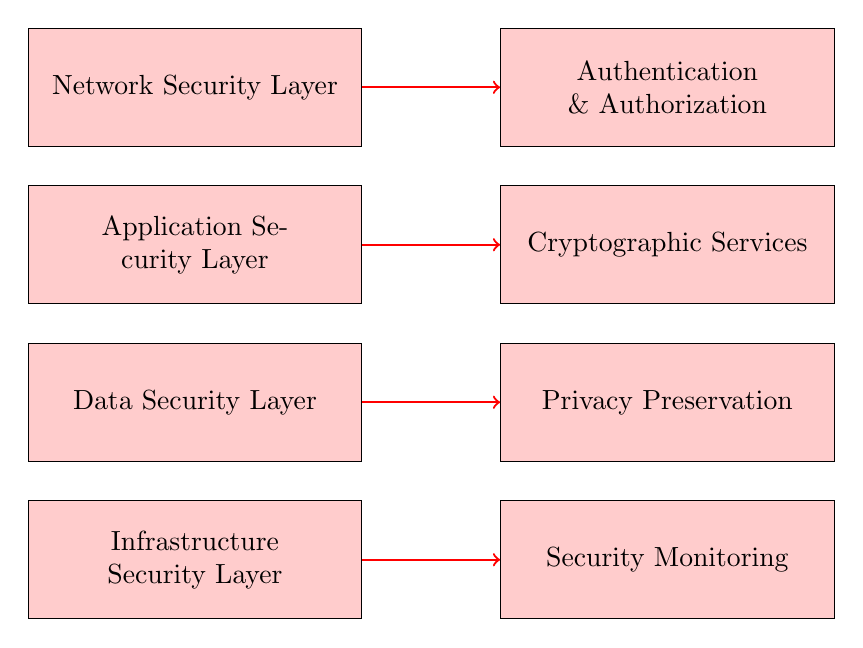
\begin{tikzpicture}[
    node distance=2cm,
    layer/.style={rectangle, draw, fill=red!20, text width=4cm, text centered, minimum height=1.5cm},
    arrow/.style={->, thick, red}
]
    % Security Layers
    \node[layer] (network) {Network Security Layer};
    \node[layer, below of=network] (app) {Application Security Layer};
    \node[layer, below of=app] (data) {Data Security Layer};
    \node[layer, below of=data] (infra) {Infrastructure Security Layer};
    
    % Side components
    \node[layer, right of=network, xshift=4cm] (auth) {Authentication \& Authorization};
    \node[layer, right of=app, xshift=4cm] (crypto) {Cryptographic Services};
    \node[layer, right of=data, xshift=4cm] (privacy) {Privacy Preservation};
    \node[layer, right of=infra, xshift=4cm] (monitoring) {Security Monitoring};
    
    % Connections
    \draw[arrow] (network) -- (auth);
    \draw[arrow] (app) -- (crypto);
    \draw[arrow] (data) -- (privacy);
    \draw[arrow] (infra) -- (monitoring);
\end{tikzpicture}
\caption{Multi-layered Security Architecture}
\label{fig:security-arch}
\end{figure}

\subsection{Authentication and Authorization}

The system implements robust authentication and authorization mechanisms:

\subsubsection{Multi-factor Authentication (MFA)}
\begin{lstlisting}[language=python, caption=MFA Implementation]
from cryptography.hazmat.primitives import hashes
from cryptography.hazmat.primitives.kdf.pbkdf2 import PBKDF2HMAC
import pyotp
import qrcode

class MFAService:
    def __init__(self):
        self.totp_secrets = {}
        
    def generate_secret_key(self, user_id):
        """Generate TOTP secret for user"""
        secret = pyotp.random_base32()
        self.totp_secrets[user_id] = secret
        return secret
        
    def generate_qr_code(self, user_id, secret):
        """Generate QR code for authenticator app"""
        totp_uri = pyotp.totp.TOTP(secret).provisioning_uri(
            name=user_id,
            issuer_name="FLOPY-NET"
        )
        qr = qrcode.QRCode(version=1, box_size=10, border=5)
        qr.add_data(totp_uri)
        qr.make(fit=True)
        return qr.make_image(fill_color="black", back_color="white")
        
    def verify_totp(self, user_id, token):
        """Verify TOTP token"""
        secret = self.totp_secrets.get(user_id)
        if not secret:
            return False
        totp = pyotp.TOTP(secret)
        return totp.verify(token)
\end{lstlisting}

\subsubsection{Role-Based Access Control (RBAC)}
The system implements granular RBAC with the following roles:

\begin{table}[htbp]
\centering
\caption{Security Roles and Permissions}
\label{tab:security-roles}
\begin{tabular}{|l|l|l|}
\hline
\textbf{Role} & \textbf{Permissions} & \textbf{Scope} \\
\hline
System Admin & Full system access & All components \\
\hline
FL Coordinator & Manage FL sessions & FL Framework \\
\hline
Data Scientist & Model development & FL Models, Analytics \\
\hline
Network Admin & Network configuration & SDN, GNS3 \\
\hline
Auditor & Read-only access & Logs, Metrics \\
\hline
Client Node & Participate in FL & Specific FL sessions \\
\hline
\end{tabular}
\end{table}

\subsection{Cryptographic Security}

The framework employs state-of-the-art cryptographic techniques:

\subsubsection{End-to-End Encryption}
\begin{lstlisting}[language=python, caption=E2E Encryption Implementation]
from cryptography.fernet import Fernet
from cryptography.hazmat.primitives import serialization
from cryptography.hazmat.primitives.asymmetric import rsa, padding
from cryptography.hazmat.primitives import hashes

class E2EEncryption:
    def __init__(self):
        self.private_key = rsa.generate_private_key(
            public_exponent=65537,
            key_size=2048
        )
        self.public_key = self.private_key.public_key()
        
    def encrypt_model_update(self, model_data, recipient_public_key):
        """Encrypt model update for secure transmission"""
        # Generate symmetric key
        symmetric_key = Fernet.generate_key()
        fernet = Fernet(symmetric_key)
        
        # Encrypt model data with symmetric key
        encrypted_data = fernet.encrypt(model_data)
        
        # Encrypt symmetric key with recipient's public key
        encrypted_key = recipient_public_key.encrypt(
            symmetric_key,
            padding.OAEP(
                mgf=padding.MGF1(algorithm=hashes.SHA256()),
                algorithm=hashes.SHA256(),
                label=None
            )
        )
        
        return {
            'encrypted_data': encrypted_data,
            'encrypted_key': encrypted_key
        }
\end{lstlisting}

\subsubsection{Secure Multi-party Computation (SMC)}
The system implements SMC protocols for privacy-preserving computations:

\begin{lstlisting}[language=python, caption=SMC Protocol Implementation]
import numpy as np
from typing import List, Tuple

class SecretSharing:
    def __init__(self, prime: int = 2**31 - 1):
        self.prime = prime
        
    def share_secret(self, secret: int, num_shares: int, threshold: int) -> List[Tuple[int, int]]:
        """Shamir's Secret Sharing"""
        coefficients = [secret] + [
            np.random.randint(0, self.prime) for _ in range(threshold - 1)
        ]
        
        shares = []
        for i in range(1, num_shares + 1):
            y = sum(coeff * (i ** j) for j, coeff in enumerate(coefficients)) % self.prime
            shares.append((i, y))
            
        return shares
        
    def reconstruct_secret(self, shares: List[Tuple[int, int]]) -> int:
        """Reconstruct secret from shares using Lagrange interpolation"""
        def lagrange_interpolation(x_coords, y_coords, x):
            result = 0
            for i in range(len(x_coords)):
                term = y_coords[i]
                for j in range(len(x_coords)):
                    if i != j:
                        term = term * (x - x_coords[j]) // (x_coords[i] - x_coords[j])
                result += term
            return result % self.prime
            
        x_coords = [share[0] for share in shares]
        y_coords = [share[1] for share in shares]
        return lagrange_interpolation(x_coords, y_coords, 0)
\end{lstlisting}

\subsection{Privacy-Preserving Technologies}

The framework implements advanced privacy-preserving techniques:

\subsubsection{Differential Privacy}
\begin{lstlisting}[language=python, caption=Differential Privacy Implementation]
import numpy as np
from scipy import stats

class DifferentialPrivacy:
    def __init__(self, epsilon: float = 1.0):
        self.epsilon = epsilon
        
    def add_laplace_noise(self, value: float, sensitivity: float) -> float:
        """Add Laplace noise for differential privacy"""
        scale = sensitivity / self.epsilon
        noise = np.random.laplace(0, scale)
        return value + noise
        
    def add_gaussian_noise(self, value: float, sensitivity: float, delta: float = 1e-5) -> float:
        """Add Gaussian noise for (ε,δ)-differential privacy"""
        sigma = np.sqrt(2 * np.log(1.25 / delta)) * sensitivity / self.epsilon
        noise = np.random.normal(0, sigma)
        return value + noise
        
    def privatize_gradient(self, gradient: np.ndarray, clip_norm: float = 1.0) -> np.ndarray:
        """Apply differential privacy to gradient updates"""
        # Clip gradient
        norm = np.linalg.norm(gradient)
        if norm > clip_norm:
            gradient = gradient * clip_norm / norm
            
        # Add noise
        noise = np.random.laplace(0, clip_norm / self.epsilon, gradient.shape)
        return gradient + noise
\end{lstlisting}

\subsubsection{Homomorphic Encryption}
The system supports homomorphic encryption for computation on encrypted data:

\begin{lstlisting}[language=python, caption=Homomorphic Encryption Integration]
from seal import *

class HomomorphicComputation:
    def __init__(self):
        self.parms = EncryptionParameters(scheme_type.ckks)
        self.poly_modulus_degree = 8192
        self.parms.set_poly_modulus_degree(self.poly_modulus_degree)
        self.parms.set_coeff_modulus(CoeffModulus.Create(
            self.poly_modulus_degree, [60, 40, 40, 60]
        ))
        
        self.context = SEALContext(self.parms)
        self.keygen = KeyGenerator(self.context)
        self.secret_key = self.keygen.secret_key()
        self.public_key = self.keygen.create_public_key()
        
    def encrypt_model_weights(self, weights):
        """Encrypt model weights for secure aggregation"""
        encryptor = Encryptor(self.context, self.public_key)
        encoder = CKKSEncoder(self.context)
        
        encrypted_weights = []
        for weight_layer in weights:
            plain = encoder.encode(weight_layer.flatten(), 2.0**40)
            encrypted = encryptor.encrypt(plain)
            encrypted_weights.append(encrypted)
            
        return encrypted_weights
\end{lstlisting}

\subsection{Network Security}

The networking layer implements comprehensive security measures:

\subsubsection{Network Segmentation}
\begin{itemize}
    \item \textbf{VLAN Isolation}: Separate VLANs for different system components
    \item \textbf{Firewall Rules}: Granular firewall policies between network segments
    \item \textbf{Zero Trust Network}: Verify every connection before granting access
    \item \textbf{VPN Tunneling}: Secure communication channels for remote clients
\end{itemize}

\subsubsection{Intrusion Detection System (IDS)}
\begin{lstlisting}[language=python, caption=Network IDS Implementation]
import asyncio
import json
from scapy.all import sniff, IP, TCP
from collections import defaultdict
import time

class NetworkIDS:
    def __init__(self):
        self.connection_counts = defaultdict(int)
        self.suspicious_activities = []
        self.thresholds = {
            'max_connections_per_ip': 100,
            'scan_detection_threshold': 20,
            'time_window': 60  # seconds
        }
        
    def analyze_packet(self, packet):
        """Analyze network packet for suspicious activities"""
        if IP in packet:
            src_ip = packet[IP].src
            dst_ip = packet[IP].dst
            
            # Track connection attempts
            self.connection_counts[src_ip] += 1
            
            # Detect port scanning
            if TCP in packet and packet[TCP].flags == 2:  # SYN flag
                self.detect_port_scan(src_ip, dst_ip, packet[TCP].dport)
                
            # Detect connection flooding
            if self.connection_counts[src_ip] > self.thresholds['max_connections_per_ip']:
                self.alert_ddos_attempt(src_ip)
                
    def detect_port_scan(self, src_ip, dst_ip, port):
        """Detect potential port scanning activities"""
        key = f"{src_ip}->{dst_ip}"
        if key not in self.port_scan_tracker:
            self.port_scan_tracker[key] = set()
            
        self.port_scan_tracker[key].add(port)
        
        if len(self.port_scan_tracker[key]) > self.thresholds['scan_detection_threshold']:
            self.alert_port_scan(src_ip, dst_ip)
\end{lstlisting}

\subsection{Compliance Framework}

The system implements comprehensive compliance mechanisms:

\subsubsection{GDPR Compliance}
\begin{itemize}
    \item \textbf{Data Minimization}: Collect only necessary data for FL operations
    \item \textbf{Purpose Limitation}: Use data only for specified FL purposes
    \item \textbf{Right to Erasure}: Implement data deletion capabilities
    \item \textbf{Data Portability}: Enable data export in standard formats
    \item \textbf{Consent Management}: Track and manage user consent
\end{itemize}

\subsubsection{HIPAA Compliance}
For healthcare applications:
\begin{itemize}
    \item \textbf{PHI Protection}: Encrypt all Protected Health Information
    \item \textbf{Access Controls}: Implement minimum necessary access principles
    \item \textbf{Audit Trails}: Maintain comprehensive access logs
    \item \textbf{Business Associate Agreements}: Ensure third-party compliance
\end{itemize}

\subsubsection{Compliance Monitoring}
\begin{lstlisting}[language=python, caption=Compliance Monitoring System]
class ComplianceMonitor:
    def __init__(self):
        self.compliance_rules = {
            'gdpr': {
                'data_retention_days': 730,
                'encryption_required': True,
                'consent_required': True
            },
            'hipaa': {
                'phi_encryption': True,
                'access_logging': True,
                'minimum_necessary': True
            }
        }
        
    async def check_data_retention(self):
        """Monitor data retention compliance"""
        expired_data = await self.find_expired_data()
        for data_item in expired_data:
            await self.schedule_data_deletion(data_item)
            
    async def audit_access_patterns(self):
        """Audit data access for compliance violations"""
        access_logs = await self.get_access_logs()
        for log_entry in access_logs:
            if not self.is_access_compliant(log_entry):
                await self.flag_compliance_violation(log_entry)
                
    def generate_compliance_report(self, regulation: str) -> dict:
        """Generate compliance report for specific regulation"""
        return {
            'regulation': regulation,
            'compliance_score': self.calculate_compliance_score(regulation),
            'violations': self.get_violations(regulation),
            'recommendations': self.get_recommendations(regulation)
        }
\end{lstlisting}

\subsection{Security Incident Response}

The framework includes automated incident response capabilities:

\subsubsection{Incident Detection}
\begin{itemize}
    \item \textbf{Anomaly Detection}: ML-based detection of unusual system behavior
    \item \textbf{Threat Intelligence}: Integration with threat intelligence feeds
    \item \textbf{Behavioral Analysis}: Analysis of user and system behavior patterns
    \item \textbf{Real-time Alerting}: Immediate notification of security incidents
\end{itemize}

\subsubsection{Automated Response}
\begin{lstlisting}[language=python, caption=Automated Incident Response]
class IncidentResponse:
    def __init__(self):
        self.response_playbooks = {
            'ddos_attack': self.handle_ddos,
            'unauthorized_access': self.handle_unauthorized_access,
            'data_breach': self.handle_data_breach,
            'malware_detection': self.handle_malware
        }
        
    async def handle_ddos(self, incident_data):
        """Automated DDoS response"""
        attacking_ips = incident_data['source_ips']
        
        # Block attacking IPs
        for ip in attacking_ips:
            await self.block_ip_address(ip)
            
        # Scale up infrastructure
        await self.auto_scale_services()
        
        # Notify administrators
        await self.send_alert('DDoS attack detected and mitigated')
        
    async def handle_data_breach(self, incident_data):
        """Automated data breach response"""
        # Isolate affected systems
        affected_systems = incident_data['affected_systems']
        for system in affected_systems:
            await self.isolate_system(system)
            
        # Preserve forensic evidence
        await self.create_forensic_snapshot()
        
        # Notify stakeholders
        await self.notify_breach_response_team()
        
        # Generate incident report
        report = await self.generate_incident_report(incident_data)
        await self.submit_regulatory_notification(report)
\end{lstlisting}

\subsection{Security Auditing and Testing}

The system implements continuous security assessment:

\subsubsection{Automated Security Testing}
\begin{itemize}
    \item \textbf{Vulnerability Scanning}: Regular automated vulnerability assessments
    \item \textbf{Penetration Testing}: Automated penetration testing frameworks
    \item \textbf{Code Security Analysis}: Static and dynamic code analysis
    \item \textbf{Dependency Scanning}: Analysis of third-party dependencies
\end{itemize}

\subsubsection{Security Metrics}
The system tracks various security metrics:
\begin{itemize}
    \item Mean Time to Detection (MTTD)
    \item Mean Time to Response (MTTR)
    \item Number of security incidents per month
    \item Compliance score percentages
    \item Vulnerability remediation time
\end{itemize}

This comprehensive security and compliance framework ensures that the FLOPY-NET system maintains the highest standards of security, privacy, and regulatory compliance while enabling secure federated learning operations.
